% Author: Seongjin Lee 
% Hanyang University, Seoul, Korea 
% esos.hanyang.ac.kr 
% 2016-09-20
% note: some slides are adopted from  \url{www.cs.stevens.edu/~jschauma/631A/}
% https://github.com/resourceful/lecture_sysprog/

\documentclass[newPxFont,sthlmFooter,nooffset]{beamer}
\usepackage{kotex}
%\usetheme{sthlm}
\usepackage{../beamer_template/beamerthemesthlm}
\hypersetup{pdfauthor={Seongjin Lee (insight@hanyang.ac.kr)},
            pdfsubject={Lecture Note: System Programming},
            pdfkeywords={Lecture Note, System Programming, class, undergraduate},
            pdfmoddate={D: \pdfdate},
            pdfcreator={Seongjin Lee}}

%\setbeamertemplate{footline}[text line]{%
%    \parbox{\linewidth}{\vspace*{-8pt} \insertsectionhead  \hfill\insertshortauthor\hfill\insertpagenumber}}
%\setbeamertemplate{navigation symbols}{}




\title{System Programming}
\subtitle{Week 7: Signals}
\author[SJL]{Seongjin Lee}
\institute{\href{mailto:insight@hanyang.ac.kr}{insight@hanyang.ac.kr}\\\url{http://esos.hanyang.ac.kr}\\Esos Lab. Hanyang University}
\date{2016-10-19} 

\begin{document}



\frame[plain]{\titlepage} 

\frame[t]{\frametitle{Table of contents}\tableofcontents} 


%---------------------------------------------------------



\begin{frame}[t]
  \frametitle{introduction}
This chapter covers following items
  \begin{itemize}
  \item The concept
  \item Use cases of signal
  \item The problems of earlier implementations
  \item The correct ways
  \end{itemize}

\end{frame}

\section{Signal Concepts}


\begin{frame}[t]
  \frametitle{Signal Concepts}

Every signal has a name that begins with \texttt{SIG} and it is assigned with a positive number defined in \texttt{<signal.h>}
\begin{itemize}
\item \texttt{SIGABRT}: generated when a process calls \texttt{abort} function
\item \texttt{SIGALRM}: generated when a timer set byt \texttt{alarm} function goes off
\item Different versions of \textsc{Unix} have different number of signals
\end{itemize}
\end{frame}

\begin{frame}[t]
  \frametitle{Signal Concepts}
Signal generating conditions
\begin{enumerate}
\item <1-> terminal generated signals (\texttt{DELETE} or \texttt{\^-C} on many systems) causes the interrupt signal (\texttt{SIGINT})
\item <2-> Hardware exceptions generate singals
  \begin{itemize}
  \item <2-> invalid memory reference (\texttt{SIGSEGV})
  \item <2-> I/O completed (\texttt{SIGIO})
  \item <2-> user disconnected from the system (\texttt{SIGHUP})
  \item <2-> detected by HW and the kernel is notified
  \item <2-> kernel generates the appropriate signal for the process
  \end{itemize}
\item <3-> \texttt{kill(2)} function allows a process to send any signal to another process or group (have to be owner, or the superuser)
\item <4-> \texttt{kill(1)} command sends signal to other process
\item <5-> Software conditions can generate signals
\end{enumerate}

\end{frame}

\begin{frame}
  \frametitle{Signal Concepts cont'd}
Signals are asynchronous events that occurs randomly

The process has to tell the kernel ``if and when this signal occurs, do the following''

\uncover<2->{We can tell the kernel to do one of three things}
\begin{enumerate}
\item <2-> \textbf{Ignore the signal} following two can never be ignored: \texttt{SIGKILL} and \texttt{SIGSTOP} 
\item <3-> \textbf{Catch the signal} We tell the kernel to call a customized function whenever the signal occurs
  \begin{itemize}
  \item <3-> if \texttt{SIGCHLD} signal is caught, it means child has terminated
  \item <3-> signal catching function calls \texttt{waitpid} to fetch the child's process ID and termination status
  \end{itemize}
\item <4-> \textbf{Use default action} every signal has a default action
  \begin{itemize}
  \item <4-> the default action for most signals is to terminate the process> 
  \end{itemize}
\end{enumerate}

\end{frame}

\begin{frame}[t]
  \frametitle{Signal Concepts cont'd}
  \begin{figure}[h]
    \centering
    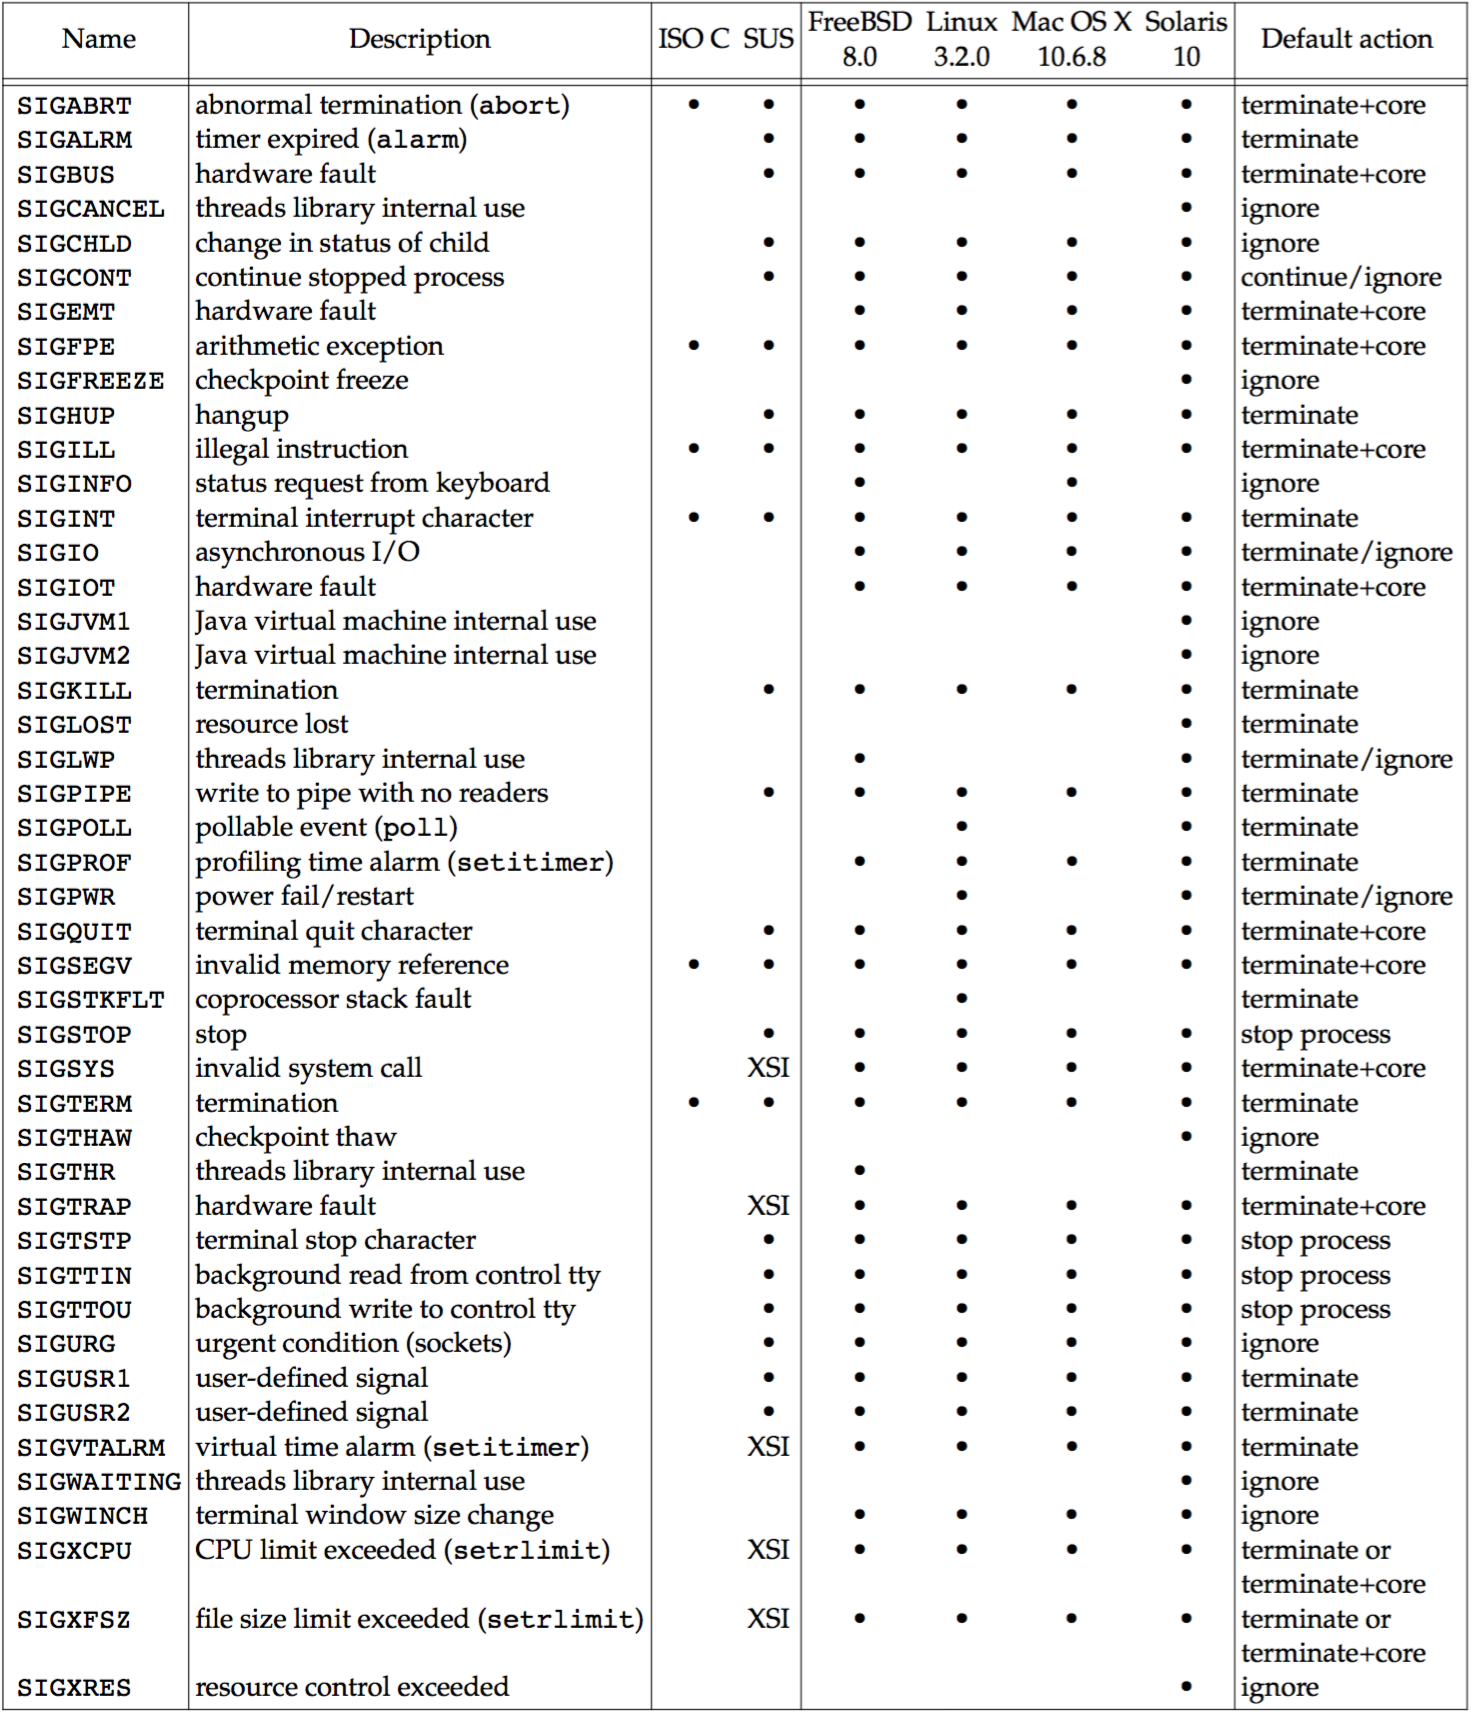
\includegraphics[width=\linewidth,trim={0 15cm 0 0},clip]{figure/fig10-1_unix_sig.png}
    \caption{\textsc{Unix} System signals}
  \end{figure}
\end{frame}

\begin{frame}[containsverbatim,t]
  \frametitle{\texttt{signal} Function}
\begin{codedef}
#include <signal.h> 
void (*signal(int signo, void (*func)(int)))(int); 
// Returns: previous disposition of signal (see following) if OK, SIG_ERR on error
\end{codedef}

\begin{itemize}[ ]
\item \texttt{signo} is name of the signal from the Table 10.1
\item \texttt{func} is
  \begin{itemize}
  \item \texttt{SIG\_IGN} : to ignore the signal
  \item \texttt{SIG\_DFL} : to use the default value
  \item address of a function to be called when the signal occurs---they are called \textit{signal handler} or \textit{signal-catching function}
  \end{itemize}
\end{itemize}
\end{frame}


\begin{frame}[fragile,containsverbatim,allowframebreaks,t]
  \frametitle{Signal Exmple Code: \texttt{codes/usr\_sig.c}}
\lstinputlisting[lineskip=0pt]{codes/usr_sig.c}
\end{frame}



\begin{frame}[containsverbatim,t]
  \frametitle{Signal Exmaples}
invoke the program in the background and use \texttt{kill(1)} to send signal
\begin{codedefnb}
James@maker:codes$ ./usr\_sig &
[2] 4987
James@maker:codes$ kill -USR1 4987
received SIGUSR1
James@maker:codes$ kill -USR2 4987
received SIGUSR2
James@maker:codes$ kill -HUP 4987
received SIGHUP
James@maker:codes$ kill -INT 4987
[2]+  Interrupt: 2            ./usr\_sig 
James@maker:codes$
\end{codedefnb}
\end{frame}




\begin{frame}[t]
  \frametitle{\texttt{signal} Function}
Process creation
\begin{itemize}
\item When a process calls \texttt{fork}, the child inherits the parents signal disposition
\item Child starts off with copy of the parent's memory image
\item the address of a signal-catching function has meaning in the child
\end{itemize}
\end{frame}



\section{The problem}

\begin{frame}[containsverbatim,t]
  \frametitle{Unreliable Signals}
In earlier versions of \textsc{Unix} system, signals were unreliable

\begin{enumerate}
\item <1-> signals get lost: signal occurs and the process never know about it
\item <2-> window of time---after the signal has occured, but before the call to \texttt{signal} in the signal handler---when the interrupt signal could occur another time. The second signal would cause the default action to occur (terminate the process)
\item <3-> little control over a signal: unable to turn a signal off when it didn't want the signal to occur. All it can do is to catch or ignore the signal.
\end{enumerate}
\end{frame}

\begin{frame}[containsverbatim,t]
  \frametitle{Interrupted System Calls cont'd}
The slow system calls are those that can block forever
\begin{itemize}
\item reads (for pipes, terminal devices, and network devices) that can block the caller
\item writes that can block the caller forever if the data can't be accepted immediately
\item open on a certain file types (terminal device) that block the caller until some condition occurs
\item the \texttt{pause} and \texttt{wait} function
\item certain \texttt{ioctl} operations
\item some of interprocess communication function
\end{itemize}

\end{frame}

\begin{frame}[containsverbatim,t]
  \frametitle{Interrupted System Calls cont'd}
The problem with interrupted system calls is that error returns must be explicit

\begin{codedef}
again:
    if ((n = read(fd, buf, BUFFSIZE)) < 0 ) {
        if (errno == EINTR)
            goto again; /* just an interrupted system call */
        /* handle other errors */
    }
\end{codedef}

The solution of 4.2BSD was to introduce the automatic restaring of \texttt{ioctl}, \texttt{read}, \texttt{readv}, \texttt{write}, \texttt{writev}, \texttt{wait}, and \texttt{waitpid}

\end{frame}



\begin{frame}[containsverbatim,t]
  \frametitle{Reentrant Functions}
  
\end{frame}



\section{Use cases of signal}



\begin{frame}[containsverbatim,t]
  \frametitle{SIGCLD Semantics}
  
\end{frame}



\begin{frame}[containsverbatim,t]
  \frametitle{Reliable-Singnal Teminology and Semantics}
  
\end{frame}


\begin{frame}[containsverbatim,t]
  \frametitle{\texttt{kill} and \texttt{raise} Functions}
  
\end{frame}



\begin{frame}[containsverbatim,t]
  \frametitle{\texttt{alarm} and \texttt{pause} Functions}
  
\end{frame}



\begin{frame}[containsverbatim,t]
  \frametitle{Signal Sets}
  
\end{frame}


\begin{frame}[containsverbatim,t]
  \frametitle{\texttt{sigprocmask} Function}
  
\end{frame}


\begin{frame}[containsverbatim,t]
  \frametitle{\texttt{sigpending} Function}
  
\end{frame}



\begin{frame}[containsverbatim,t]
  \frametitle{\texttt{sigaction} Function}
  
\end{frame}


\begin{frame}[containsverbatim,t]
  \frametitle{\texttt{segsetjmp} and \texttt{siglongjmp} Functions}
  
\end{frame}


\begin{frame}[containsverbatim,t]
  \frametitle{\texttt{sigsuspend} Function}
  
\end{frame}



\begin{frame}[containsverbatim,t]
  \frametitle{\texttt{abort} Function}
  
\end{frame}


\begin{frame}[containsverbatim,t]
  \frametitle{\texttt{system} Function}
  
\end{frame}


\begin{frame}[containsverbatim,t]
  \frametitle{\texttt{sleep}, \texttt{nanosleep},  and \texttt{clock\_nanosleep} Functions}
  
\end{frame}


\begin{frame}[containsverbatim,t]
  \frametitle{\texttt{sigqueue} Function}
  
\end{frame}


\begin{frame}[containsverbatim,t]
  \frametitle{Job-Control Signals}
  
\end{frame}



\begin{frame}[containsverbatim,t]
  \frametitle{Signal Names and Numbers}
  
\end{frame}

%---------------------------------------------------------
\section{Last Words}

\begin{frame}[t]
  \frametitle{Last Words}
\begin{itemize}
\item Prepare for Exam
\end{itemize}
\end{frame}

\end{document}
